%\documentclass{buthesis_p}         %Default is author-year citation style
\documentclass[numbib]{buthesis_p}  %Gives numerical citation style
%\documentclass[twoadv}{buthesis_p} %Allows entry of second advisor
% \usepackage{graphics}             %Select graphics package
\usepackage{graphicx}             %
\usepackage{amsthm}               %Add other packages as necessary
\usepackage{amsmath}               %Add other packages as necessary
\usepackage{amssymb}
\usepackage[usenames]{color}               %Add other packages as necessary
\usepackage{subcaption}
\usepackage{multicol}
\usepackage{vwcol}
\usepackage{needspace}
\usepackage{bibentry}
% \usepackage[backend=biber]{biblatex}
% \addbibresource{bibliography.bib}\usepackage{tikz}
\usepackage{tikz}
\usetikzlibrary{shapes}
\def\checkmark{\tikz\fill[scale=0.4](0,.35) -- (.25,0) -- (1,.7) -- (.25,.15) -- cycle;}
\def\circle{
\begin{tikzpicture}[scale=2]
                \coordinate [label=left:$O$] (O) at (0,0);
                \coordinate [label=right:$$] (A) at (0,1);
                \coordinate [label=right:$$] (B) at (0,0);
                \node[draw,circle through=(A)] at (O){};
                \filldraw[black](A) circle (1pt);
        % \draw[fill,color=red](0,0) circle (2cm and 2cm);
        % \draw[fill,color=white](0,0) circle (1cm and 1cm);
\draw (O)--(A);
\end{tikzpicture}}


\begin{document}
\butitle{Simulation and Theory of Antibiotic Resistant Bacteria Populations}
\author{J. Russo}
\degree{Bachelor of Science}
\department{Physics}
\advisor{Jiajia Dong}
%\advisorb{Jane Doe}              %Second advisor if necessary
\chair{Michele Thornley}
\maketitle

\setlength{\columnseprule}{1pt}
% \def\columnseprulecolor{\color{blue}}

\newcommand\blfootnote[1]{%
  \begingroup
  \renewcommand\thefootnote{}\footnote{#1}%
  \addtocounter{footnote}{-1}%
  \endgroup
}

% Sec B.4, B.5
% http://www.bucknell.edu/current-student-resources/honors-program/proposal-preparation-guidelines.html

\section{Introduction}
% Short description of goals of project
% "Understandable to an educated non-specialist in that field"
The threat of antibiotic resistance, even amongst currently well-controlled diseases,
is becoming increasingly prevalent. In order to combat this rising phenomenon, %#TODO: word choice?
we must first understand the conditions that allow emerging antibiotic resistant
bacteria populations to dominate antibiotic sensitive populations. A dominant
mechanism of intercellular transmission of antibiotic resistance is through
transfer of plasmids encoding for antibiotic resistance \cite{transfer}.

% Plasmid overview
In our work we plan to focus on two main methods of plasmid transfer
 between cells, namely transformation and conjugation. Both
processes involve plasmids, which are small, independently replicating pieces %TODO: Word choice?
of genetic material. We specifically consider plasmids including DNA segments
encoding for antibiotic resistance. %TODO: Necessary to say?
Incorporating a plasmid's genetic material actually has a directly negative impact on
the host cell, imposing a small fitness cost\cite{fitnesscost} that manifests as an increased
reproduction time as a result of needing to transcribe %TODO: right word?
extra genetic information during reproduction. The somewhat seemingly contradictory nature
of this is sometimes referred to as the "plasmid paradox" \cite{plasmidparadox}.
However, when presented with selective pressure such as exposure to antibiotics,
plasmids become hugely beneficial to their host cells, allowing them to survive
in conditions that would otherwise kill off entire populations \cite{plasmidparadox}\cite{fitnesscost}. %TODO: 'kill off' phrasing

% Methods of plasmid transfer
Through transformation, a sensitive cell acquires a plasmid from its environment,
translating any encoded genes into its own DNA sequence. In conjugation,
a resistant cell transfers genetic material to a sensitive cell through direct
physical contact. %TODO: Do I need more detail on how this works?
%TODO: Mention that previous work has dealt with transformation?


% Well-mixed vs spatially structured
%TODO: Plan to continue exploring?
We plan to explore interactions between bacteria and plasmids in two
significantly different environments. %
%TODO: Should well-mixed and spatially-structued be broken into two separate sections?
The well-mixed environment is analogous
to a shaken mixture of bacteria suspended in a fluid in a flask, where cells are
uniformly distributed and have equal access to plasmids. The spatially-structured
case examines a situation like a biofilm, where bacteria have coalesced to form
a two-dimensional, lattice-like layer. %TODO: "Lattice-like"?
These present both the need for different simulation techniques, and vastly
different results. Though we investigate applications to a biological system,
we use mathematical and simulation frameworks which are also applicable in a wide range
of physical and chemical contexts.

\section{Project Description}

% We plan to investigate the interplay between growth of populations of both
% antibiotic sensitive (S) and resistant (R) bacteria. %TODO: do I want these S/R abbrevs?
% We will further refine a simulation %
% we have developed to model these in both well-mixed and spatially-structured
% environments by adding more complete descriptions of the effects of antibiotics,
% cell-to-cell conjugation, and cell motion. %Need more specific details here about what we're trying to do

% Reactions

\subsection{Preliminary Investigation}
Work conducted in the summer of 2016 provides preliminary results which we plan
to use as a starting point for more sophisticated simulation. We focused on
transformation as the dominant method of plasmid transfer, and examined three
primary regimes of different transformation rates $\alpha$ under which it occurs,
demonstrated in Figure \ref{fig:transf}. %TODO: Poor phrasing

% Transformation regimes
\begin{figure}[h]
\centering
\begin{subfigure}{0.3\linewidth} \centering
 \frame{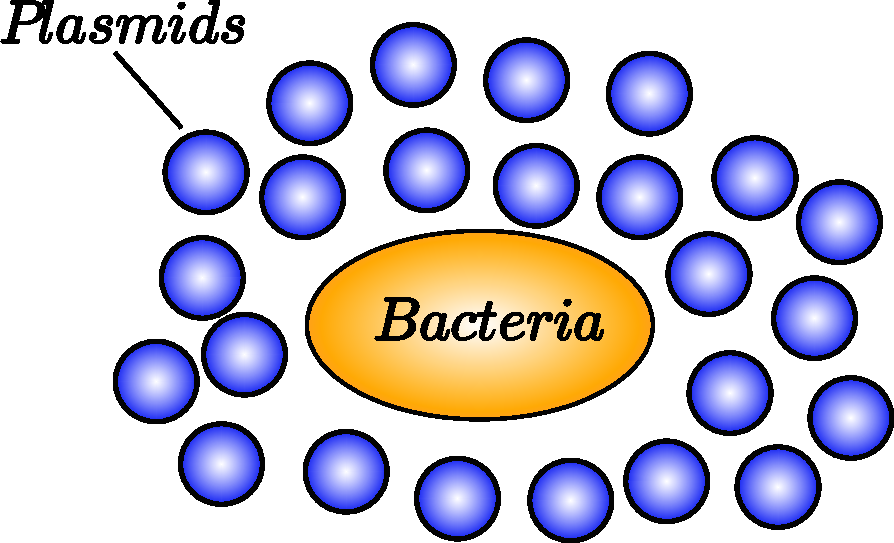
\includegraphics[scale=0.3]{./constant.pdf}}
 \caption{Plasmid abundance effectively yields a constant rate of transformation, $\alpha$.}
 \label{fig:const}
\end{subfigure}
\hspace{1ex} \vrule \hspace{1ex}
\begin{subfigure}{0.3\linewidth} \centering
 \frame{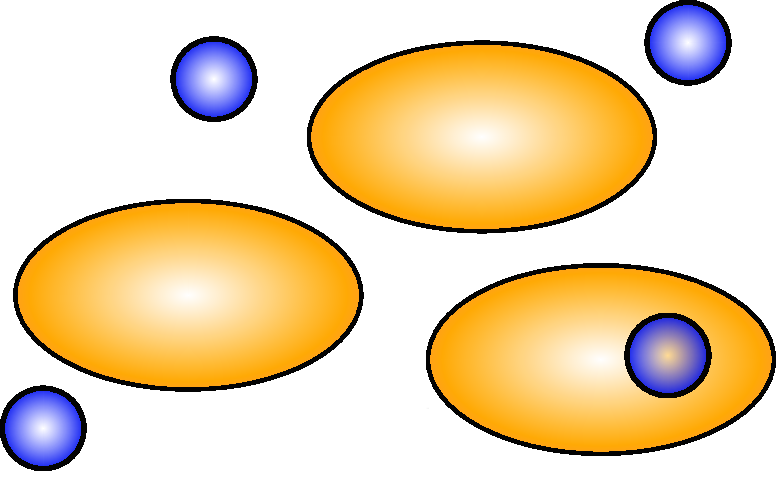
\includegraphics[scale=0.3]{./linear.pdf}}
 \caption{A fixed initial population of plasmids that are consumed by transformation
 yields the linear $\alpha$ case.}
 \label{fig:linear}
\end{subfigure}
\hspace{1ex} \vrule \hspace{1ex}
\begin{subfigure}{0.3\linewidth} \centering
 \frame{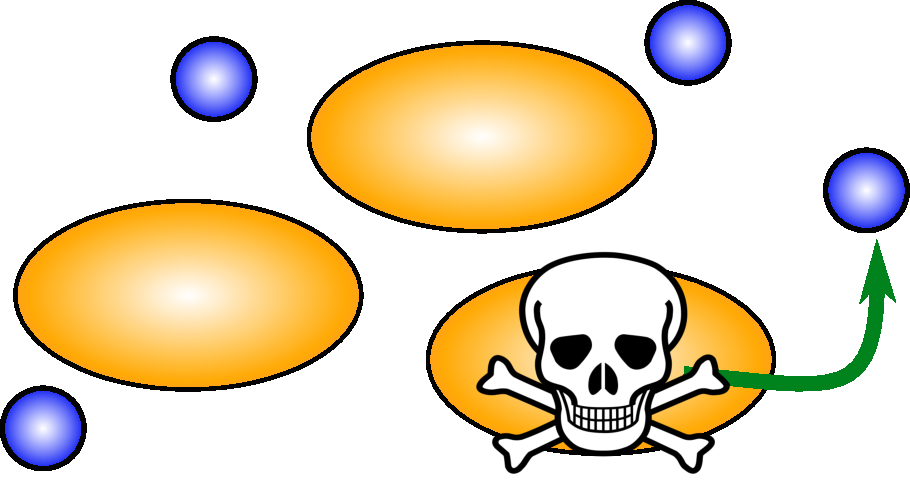
\includegraphics[scale=.3]{./recycled.pdf}}
 \caption{A feedback mechanism where dead cells return free plasmids to
 the environment defines the recycled $\alpha$ case.}
 \label{fig:recycled}
\end{subfigure}
\caption{Transformation regimes explored in preliminary research.} %TODO: Write a standalone description of these, define alpha more explicitly.
\label{fig:transf}
\end{figure}



  \subsubsection{Reactions}
In our previous research, we defined four main reactions as follows:

% \needspace{7\baselineskip}
\noindent\makebox[\textwidth][c]{
\begin{minipage}{.35\linewidth}
    \centerline{\textbf{Reactions}}
    \begin{align}
      S & \stackrel{b_S}{\rightarrow} 2S \label{rxn:sbirth}\\[3.5ex]
      S \color{red}+ P_{free}\color{black} & \stackrel{\alpha}{\rightarrow}  R \label{rxn:transf}\\[3.5ex]
      R & \stackrel{b_R}{\rightarrow} 2R \label{rxn:rbirth}\\[3.5ex]
      R & \stackrel{\delta}{\rightarrow} \varnothing \color{blue} + P_{free} \color{black} \label{rxn:death}
    \end{align}
  \end{minipage} \quad\vrule\quad
  \begin{minipage}{.6\linewidth}
  \centerline{\textbf{Equations}}
\begin{align}
  \frac{dS}{dt} & = b_S \left(1 - \frac{S + R}{K}\right)S - \alpha
    \color{red}\left( \frac{P_{f}}{P} \right)
    \color{black} S \label{eqn:sbirth} \\[1.5ex]
%
  \frac{dR}{dt} & = b_R \left(1 - \frac{S + R}{K}\right)R + \alpha
  \color{red}\left( \frac{P_{f}}{P} \right)
  \color{black} S - \delta R \label{eqn:rbirth}\\[1.5ex]
%
  \color{red} \frac{dP_{f}}{dt} & \color{red} = -\alpha \left( \frac{P_{f}}{P} \right) S
  \color{blue} + \delta R \label{eqn:pfree}\\[1.5ex]
%
  \color{red}\frac{dP}{dt} & \color{red}= b_R \left( 1 - \frac{S + R}{K} \right) R \label{eqn:ptot}
\end{align}
\end{minipage}
}
\begingroup
  \captionof{table}{The reactions and associated differential equations modeled
  by our simulation. Highlighted in red and
  blue are terms specific to the \color{red}linear \color{black}
  and \color{blue}recycled \color{black} $\alpha$ cases, respectively.}
\endgroup

 %TODO: This isn't a table
%TODO: This isn't clear either, blue terms apply to linear too, not just recycled
%TODO: Detail
%TODO: Formatting


%TODO: How to segue into these descriptions?
\indent These reactions describe S cell
birth, transformation, R cell birth, and R cell death respectively. The additional
colored terms are illustrative of the three different transformation regimes. The added
$P_{free}$ term in Equation \ref{rxn:transf} defines the linear $\alpha$ case
shown in Figure \ref{fig:linear}, where a
free plasmid from the environment must be consumed for transformation. Additionally,
adding a free plasmid to the products of Equation \ref{rxn:death} describes the
recycled $\alpha$ case.

On the equation side, the constant $\alpha$ case is described by just two
equations, Eqn. \ref{eqn:sbirth} and Eqn. \ref{eqn:rbirth}, which describe
the S and R population growth rates. In order to describe the linear case it is
necessary to now track not only the number of free plasmids, but also the number
of total available plasmids, which will now be increasing as a result of what
we refer to as symmetric reproduction. Essentially, when Equation \ref{rxn:rbirth}
occurs, an additional R cell is created without consuming a free plasmid, and
so the total number of plasmids in the system increases by one. An equation for
the recycled case is obtained by simply incrementing free plasmid
count proportionally with R cell death.

  \subsubsection{Simulation overview}
We implementated the Kinetic Monte Carlo (K.M.C.) method (or Gillespie Algorithm)
to perform our simulations. This is an
algorithm that was initially developed for simulating stochastic chemical
processes. However, the K.M.C. method is agnostic
to the actual quantities being simulated, relying only on having a set of reactions
that occur with given propensities. This means that our simulation methods are not
specific to what we're simulating, just to the reactions and population sizes, and
therefore can be generalized to a wide range of systems. Furthermore, K.M.C. randomly samples time
step length from an exponential distribution. Since one reaction occurs per time step,
adjusting the time step length allows the algorithm to adjust for a larger
number of particles, which would have reactions occuring more frequently, and
conversely to a smaller number of particles, which would have less frequent reactions.

\begin{figure}
  \centerline{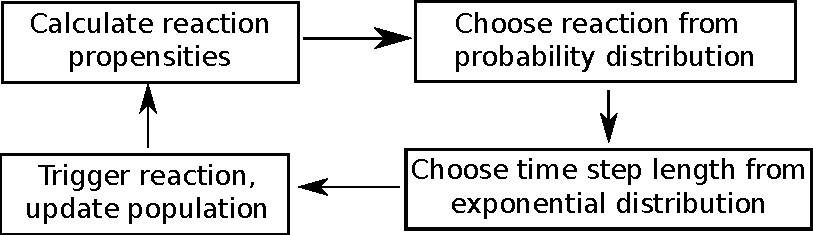
\includegraphics[width=.7\linewidth]{graphics/gillespie.pdf}}
  \caption{Basic diagram of Gillespie Algorithm. Reactions are randomly selected
  based on propensities, which are calculated using their rates of reaction.
  Time step length is chosen from an exponential distribution such that it adjusts
  itself based on the number of particles being simulated. More details are
  available in Appendix \ref{algDetails}.}
\end{figure}

  \subsubsection{Preliminary results}
  % Next steps/segue into proposal for new work
  We obtained results for all three transformation mechanisms in the well-mixed case.
  Most notably, we discovered a transition
  point where for certain ranges of birth rate and $\alpha$ values, population
  dominance switches from the S to R population. We found that this transition
  point is heavily dependent on the transformation mechanism, and very minimally
  sensitive to the actual value of $\alpha$. Furthermore, the linear case tends
  to population extinction, with the most dynamic behavior of the three.

\subsection{Proposed Research}
% Detail objectives (additions to simulation)
% Antibiotics
% Conjugation
% Diffusion (spatially-structured)
We plan to continue this research by expanding our simulation to model the
populations more accurately. Specifically, we plan to accomplish this by incorporating
three main new elements, and studying their impacts.

\begin{tabular}{l || c | c | c | c}
& Transformation & Conjugation & Diffusion & Antibiotic Exposure \\ \hline
Well-Mixed & \checkmark & \circle & $\times$ & \\ \hline
Lattice & ? & $\times$ & $\times$ & \\ %\hline
\end{tabular}
\captionof{table}{This shows aspects of our research we either have completed or will
study. Well studied regimes are denoted by a checkmark, an empty circle indicates
an area we will explore, and a shaded circle represents an area we have begun
to explore, but have not fully analyzed. }

\subsubsection{Conjugation}
Firstly, we plan to introduce a new reaction for cell-to-cell conjugation as in
Equation \ref{rxn:conjug}.
\begin{equation}
  S + R \rightarrow 2R
  \label{rxn:conjug}
\end{equation}
Presently, we consider transformation as the exclusive mechanism of plasmid transport.
However, conjugation is also a common process, and may introduce interesting system
dynamics as populations of R cells bordering groups of S cells now have a mechanism
to directly transfer plasmids encoding antibiotic resistance to them. %TODO: PHRASING

To successfully study the effects of conjugation on our system, we will also
incorporate it into our mathematical model to obtain predictions for behavior.
To do this, we will need to add an additional term to Equations \ref{eqn:sbirth}
and \ref{eqn:rbirth}. %TODO: more specifics?

\subsubsection{Diffusion}
Presently, in the spatially-structured case we do not include any model of
cellular motion, instead assuming that a cell stays at its initial lattice site
for its entire lifetime. As a result, populations can only spread out by reproduction,
which randomly places daughter cells at adjacent lattice sites. In reality,
bacterial cells are capable of individual motion. We plan to simulate
this using a simple diffusion model, where populations will attempt to slowly spread
out of high concentration areas into lower concentration areas. This will involve
adding a new reaction which will move a random cell. This is specific to the
lattice case, so we will not be able to mathematically model it. %TODO: phrasing?

\subsubsection{Antibiotic Exposure}
The crux of this research is determining which conditions lead to and which conditions mitigate
antibiotic-resistant bacteria population dominance. An important consideration
in this is if a population is dosed with antibiotics early on when each
population numbers relatively few, this could lead to an early extinction of
sensitive cells, even in situations that would otherwise tend to sensitive
cell dominance. In order to better understand this potential effect, we plan to
simulate different regimes of antibiotic exposure to see how they affect population
dominance over time. %TODO: Specifics, and how do we intend to do this?

\section{Contribution}
% My own contribution to the project
% Developing simulation
My role in this project will involve work on both the computational and theoretical
aspects of our research. In our work from the summer of 2016, I developed two
computer simulations we used to study the populations, one for the well-mixed case,
and one for the spatially-structured case. I was responsible not
only for programming the simulation, but for implementing a number of optimizations
without which the simulation would have taken too long to run to gather meaningful
data. These were exceptionally useful in the spatially-structured case due to the
hugely increased computational complexity.
I have acquired experience in software development and simulation through a number
of projects outside of my research at Bucknell, including work on parallelized
multiprocessing and simulation development. As our project becomes increasingly
technically demanding, I will continue to apply my unique experience in this area to further develop
our simulation and add the more detailed and accurate features mentioned above to it.
These improved simulations will allow my advisor to conduct more in-depth study
for her own research on bacterial population dynamics.

Additionally, in our summer research I helped develop the differential equations
that characterize the populations. I proposed and developed the equations
for the free plasmid and total plasmid numbers, which were necessary for both
the linear and recycled case. I also used these models to generate and analyze predicted
population trajectories\cite{nldynamics}, which I verified using my simulation. I plan to apply
similar techniques as we expand our simulation, and believe this will be
increasingly useful as our population dynamics become more complex.

\section{Significance}
% Ubiquity of antibiotic resistance
% Usefulness in combatting
Antibiotic resistance is a rising epidemic the World Health Organization
describes as "so serious that it threatens the achievements of modern medicine."\cite{who}
Antibiotic resistant mutations of currently well-contained diseases such as
tuberculosis and bacteria like E. coli present us with strains of these
familiar ailments that can be completely nonresponsive to contemporary treatments.
Startlingly, the WHO also states that study on antibiotic resistance is
"neither coordinated nor harmonized", leaving us with
"many gaps in information on bacteria of major public health importance."\cite{who}

Our next steps will, among other things, %TODO: this is vague
give us deeper insight into how antibiotic dosing affects the dynamics of
population growth. This will allow us to compare relative effectiveness of
different antibiotic dosing regiments currently being used for treatment.

An in-depth understanding of this phenomenon is an essential first step towards
being able to combat it. Our research provides a means by which we can begin
to model how these populations develop, and what factors are most critical
in whether sensitive or resistant bacteria dominate the population. By
making a more detailed, refined model, we improve our ability to be able
to hone in on certain factors. Already we have obtained significant,
meaningful results, such as finding that in the parameter ranges we
have considered, the fitness cost imposed
by the plasmids on the cell is only a second-order effect, and does not significantly
affect dominance.

As I go forward into graduate school and more research, this project will give me
invaluable experience in the research process, and in conducting simulation and
modelling of complex problems with real-world consequences.
% This project will be a formative part of my undergraduate research experience,
% and an excellent springboard into larger scale research in graduate school. As
% I intend to continue into graduate school to work towards my doctorate, having
% an opportunity like this will help jump start my research career. It will provide me
% with a wealth of critical, early, firsthand experience in the process I plan to spend my
% career pursuing. It will help me continue to develop a repertoire of skills that
% will continue to serve me for years to come.

%%%%Use following line if bibtex is being used.
%\bibliography{samplebib.bib}


\newpage
%%%Use following if references are being entered by hand.
\begin{thebibliography}{99}
% \bibitem[Rieger(2012)]{rieger}H.~Rieger, ``Kinetic Monte Carlo''
% Lecture slides (2012).

\bibitem {transfer} Svara, Fabian and Daniel J Rankin. "The Evolution Of Plasmid-Carried Antibiotic Resistance".
BMC Evol Biol 11.1 (2011): 130. Web. 8 Sept. 2016.

\bibitem {fitnesscost} Vogwill, Tom and R. Craig MacLean. "The Genetic Basis Of %
The Fitness Costs Of Antimicrobial Resistance: A Meta-Analysis Approach". Evol Appl 8.3 (2014): 284-295. Web. 8 Sept. 2016.

\bibitem {plasmidparadox} MacLean, R. Craig and Alvaro San Millan.
"Microbial Evolution: Towards Resolving The Plasmid Paradox". Current Biology 25.17 (2015): R764-R767. Web. 8 Sept. 2016.

\bibitem {gillespie} Gillespie, Daniel T.
"A General Method for Numerically Simulating the Stochastic Time Evolution of Coupled Chemical Reactions".
Journal of Computational Physics (1976). 22 (4): 403–434. doi:10.1016/0021-9991(76)90041-3.


\bibitem {nldynamics} Strogatz, Steven H. Nonlinear Dynamics And Chaos.
Cambridge, MA: Westview Press, 2000. Print.

\bibitem {who} World Health Organization, ``Antimicrobial resistance: global report on surveillance ''
World Health Organization Press (2014).

\end{thebibliography}


\newpage
\appendix
\section{\\Gillespie Algorithm details} \label{algDetails}

\begin{enumerate}
  \item Initialize simulation
  \item Calculate propensity $a$ for each reaction
  \item Choose reaction $\mu$ according to the distribution
    $$\text{P(reaction }\mu) = a_\mu / \sum_{i}a_i$$ %TODO: is this formatting ok?
  \item Choose time step length $\tau$ according to the distribution
    $$\text{P}(\tau)=\left(\sum_i a_i\right) \cdot \exp{\left(-\tau \sum_i ai\right)}$$
  \item Update populations with results of reaction
  \item Go to Step 2
\end{enumerate}
\blfootnote{See Gillespie (1976) for more details.\cite{gillespie}}
\newpage

\end{document}
